% Chapter Detector 

\chapter{Collider and Detector} \label{chap:2}
%http://iopscience.iop.org/article/10.1088/1748-0221/3/08/S08004/pdf

\section{Large Hadron Collider}%P29
Large Hadron Collider (LHC) is located at Geneva region about 100 meters underground, built and operated by European Organization for Nuclear Research, CERN. 
Its circumference is 27-km-long, and two proton beams in which the energy of each proton is 6.5 TeV produce collisions at center-of-mass energy reaching 13 TeV in 2015. 
LHC is the largest collider in the world, both in size and in center-of-mass energy.
Besides, LHC also provides heavy-ion collision to include the study of the behavior of quantum chromo dynamics, QCD, under high-density parton momentum fraction and the study of the properties of gluon-quark plasma, which is thought to constitute the universe for few $\mu$s after the Bing Bang~\citep{Heavyions}. 
When it operates, the intervals between proton bunch crossing is 25 ns, that is to say,  4 $\times 10^7$ events are produced per second. 
Besides, an average of 20 inelastic collisions will be produced in a single bunch crossing.
It is undoubtedly a challenging requirement on technique not only to reduce the number of events recorded by triggers but also to alleviate the effect by inelastic collision that cause pile-ups.

\section{The Compact Muon Solenoid Detector}

As one of the detectors of the LHC, the Compact Muon Solenoid Detector, CMS~\citep{CMSDetector}, shares the same aims of the LHC.
Basically, it will elucidate the physical properties of the Higgs boson whose mass is around 125 GeV, and it will also test the mathematical consistency of Standard Model, SM, at TeV scale.
People also hope to find new physic beyond SM where Supersymmetry and Extra Dimension is often being considered. The latter necessitates the finding of graviton in TeV scale.
All researches need a delicate design of a detector, including good charged particle reconstruction to trace the vertex, good EM energy resolution, and good measurement of missing transverse momentum and mass resolution.
\begin{itemize}
\item The tracker: The high granularity tracker at inner detector can well reconstruct the trace of charged particles. It is also indispensable for identifying b-flavored jets and $\tau$.  
\item The muon chamber: The muon chamber combined with tracker information under the magnetic field of opposite direction can  interpolate together to reduce mismatching rate in muon reconstruction, to enhance precision of measurement on high transverse momentum muons, and to identify the cosmic muons from outside of the detector.
\item The calorimeters: The calorimeters facilitate the shower and measure the energy of post-shower particles. The information will further be clustered into the energy corresponding to their mother particles.
\end{itemize}

\begin{figure}[t]
  \begin{center}

    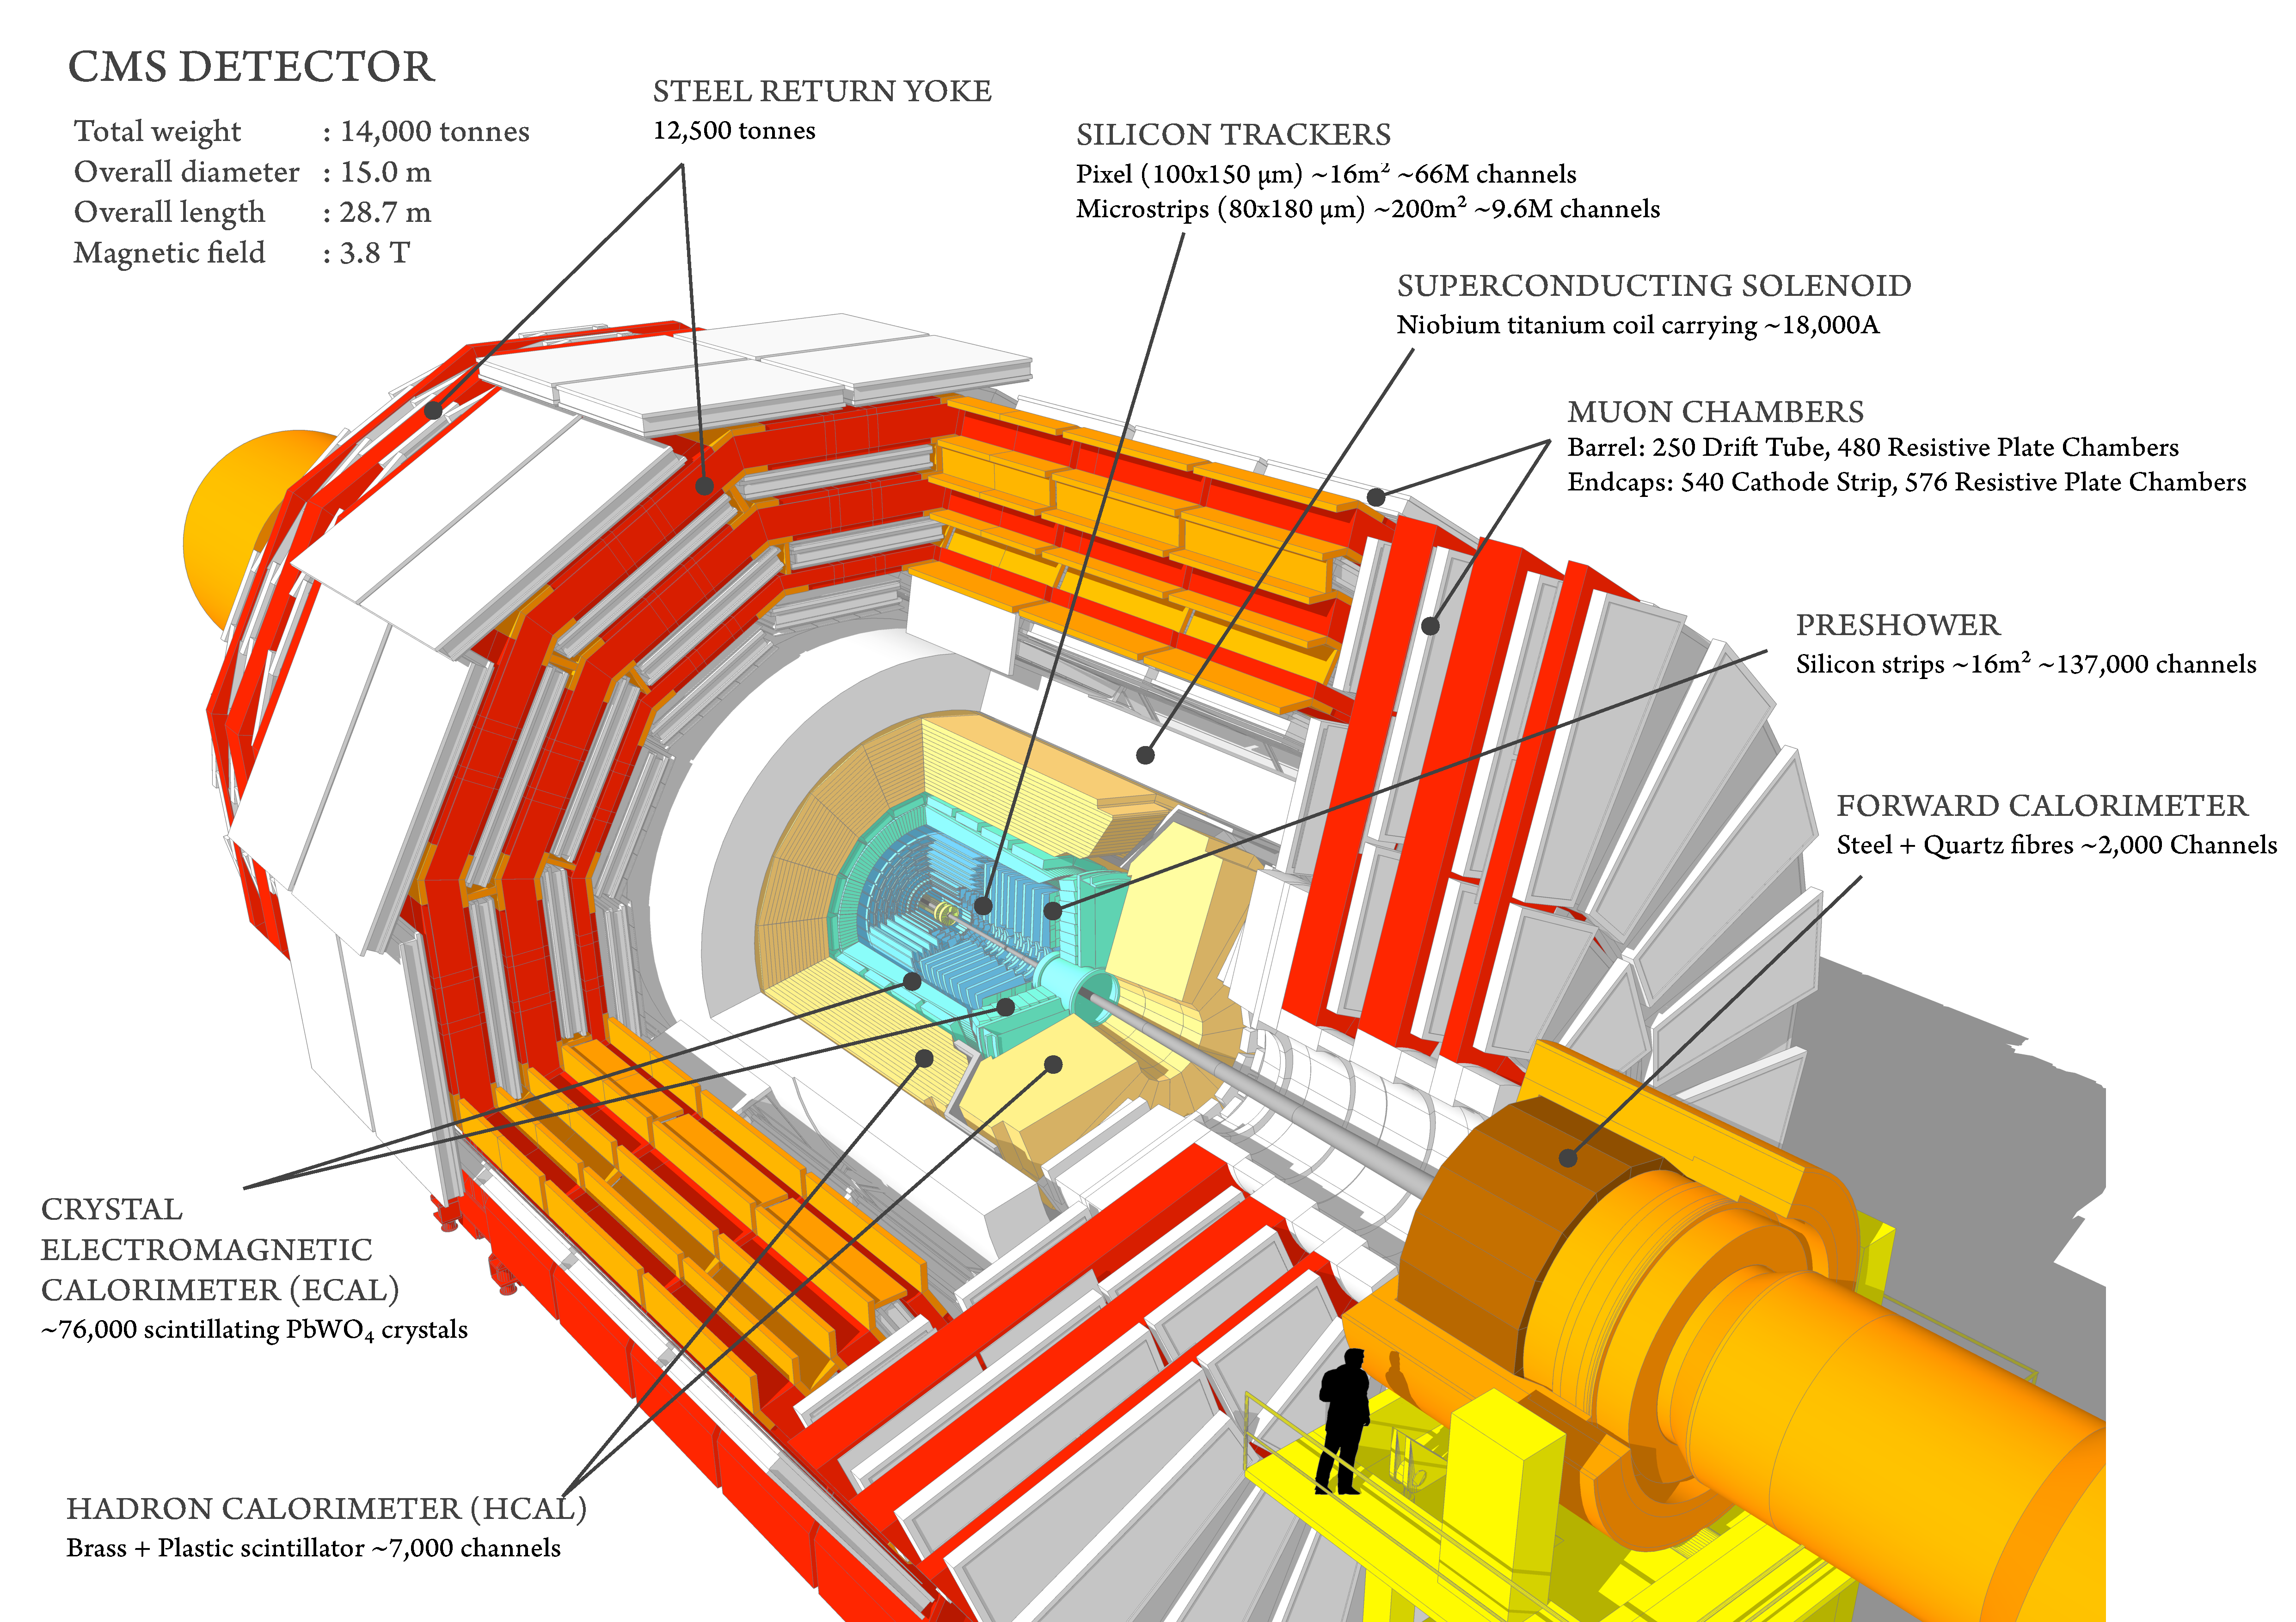
\includegraphics[width=0.5\textwidth]{Figures/cms_160312_02.pdf} 
    \end{center}
  \caption{The three-dimension sketch-up image of the CMS detector~\citep{CMSImage}.}
\end{figure}

\subsection{Detector Kinematics} 
To better describe the geometry of the detector, a set of convention is adopted. The z axis is along the beam line, and the positive direction points to the proton beam moving in the counter-clockwise direction. The x axis points to the center of the LHC circle. The xy plane is perpendicular to z axis and can be described by $\phi $:
\begin{equation} \label{eq1}
\begin{split}
x=rcos\phi, y=rsin\phi,
\end{split}
\end{equation}
where $\phi$ is the azimuthal angle, r is the distance from the z axis on xy plane. The variable rapidity y is related to the angle $\theta$ between one momentum vector and the z axis. The difference of rapidity is invariant under boosts along the z axis. When particles travel near the speed of light, its mass is negligible. Hence, $E$ $\thickapprox$ $|\vec{p}|$ and rapidity could be approximated by pseudo rapidity $\eta$ $\thickapprox$ y, while $E$ = $|\vec{p}|$ for a massless particle.
\begin{equation} \label{eq1}
\begin{split}
y = \frac{1}{2} ln( \frac{E+p_z}{E-p_z} ), \eta = \frac{1}{2} ln( \frac{|\vec{p}|+p_z}{|\vec{p}|-p_z} ) = -log[tan(\theta /2)]
\end{split}
\end{equation}

\subsection{Magnet System} 
In order to have a good resolution for charged particles in the trackers, magnetic field must maintain to bend the tracks of charged particles. 
Providing the magnetic field of CMS, the superconducting solenoid is installed between the calorimeters and muon chambers with a diameter of 6.3 m, length of 12.5 m, and mass of 200 t. 
Designed to have 3.8 T magnetic field at the center of the detector along positive z direction, the solenoid uses four layers based on the Ampere-turn (41.7MA-turn) and made of aluminum alloy.
The width of one layer is far less than its counterpart of other detectors, and its lower limit is restricted by the magnetic pressure and the material property of aluminum.
It also breaks the convention, for that the magnetic stress is shared between itself and the outer mandrels. 
The yoke whose proposes are guiding the magnetic field and absorbing particles except muons and neutrinos is composed of five barrel wheels and 6 endcap disks~\citep{yoke}. 
Besides, to avoid the "quench back" effect, where the eddy currents induced in outer mandrels heat up the coil above superconducting critical temperature, 
a protecting circuit is designed and worked by either fast discharge or slow discharge through dumping. 

\subsection{Tracker Detector} 
Having precisely-reconstructed primary and secondary vertices, the Tracker detector is designed to be at innermost part of the CMS detector.
It needs to be fast enough to collect data between 25 ns interval of bunch crossing and high granularity enough to identify the trajectories. 
Two kinds of tracker detector are used for different purposes, the pixel trackers and the strip trackers. 
While the former is better at determining three dimensional space and at enduring the radiation dose, 
the latter covers larger total area since it costs less per area. 
There are three cylindrical pixel detectors at radii of 4.4, 7.3 and 10.2 cm and two disks of pixel detectors at |z| of 34.5 and 46.5 cm on each side of the interaction point. 
They together give coverage to pseudo rapidity |$\eta $| $<$ 2.5 and an area of about 1 $m^2$ with total 66 million pixels whose size is 100 $\times$ 150 $\mu m^2$ each. 
The strip detectors are separated into several subsystems. The Tracker Inner Barrel and the Tracker Inner Disk (TIB/TID) at radii extending to 55 cm together, composing 4 layers and 3 disk on each side, 
provide four $r-\phi $ measurements with resolution of 23 $\mu m$ and of 35 $\mu m$ by the first two layers and the others respectively. 
Tracker Outer Barrel (TOB) ranges toward radius of 116 cm and performs six $r-\phi $ measurements with resolution of 53 $\mu m$ and of 35 $\mu m$ by the first four layers and the others respectively.
In addition, Tracker EndCap (TEC) gives another 9 measurements on $\phi $ by its nine layers installed at 124 cm $<$ |z| $<$ 282 cm.
 
\subsubsection{Pixel Trackers}
%https://twiki.cern.ch/twiki/pub/Main/UndergradElog2014/pixelDetectors.pdf
The pixel trackers constitutes of pn-junctions operated in depletion. 
When particles pass depletion zone, induced electron-hole pairs will produce signal current and further be amplified and read out. 
To take the high-density radiation dose into account, a n$^+$-doped electrodes in n-doped substratrate design is chosen as sensor. 
Another advantage of the n-on-n concept is that a guard ring can be made around the sensor to prevent voltage breakdown in air (1.2V/$\mu $m). 
The isolation between electrodes prevents electrodes from shortening after radiation. Open p-stop and moderate p-spray are isolation designs implemented on disks and barrel respectively~\citep{PixelD}.

\subsubsection{Strip Trackers}
The elements in the trackers are single-sided p-on-n silicon micro-strip sensors. 
Besides, the six-inch wafers are used instead of four-inch wafers to reduce the cost. 
As the built-on surface charge of $\langle$100$\rangle$ crystal orientation of n substratrate is smaller than $\langle$111$\rangle$ one, 
the $\langle$100$\rangle$ is chosen to maintain the capacitance after irradiation. The $\langle$xyz$\rangle$ is the sign used in solid state physics, which represents the direction of the plane of a crystal. To clarify, $\langle$100$\rangle$ means the first plane intercepting the x, y, and z-axis at 1, 0, and 0 respectively. Other planes are perpendicular to this plane and have distance by $\sqrt{1^2+0^2+0^2} \times$ n. Following the same rule, the first plane in $\langle$111$\rangle$ crystal intercepts the x, y, and z-axis at 1, 1, and 1 respectively. Other planes are perpendicular to this plane and have distance by $\sqrt{1^2+1^2+1^2} \times$ n.

\subsection{Electromagnetic Calorimeter} 
%118
The electromagnetic calorimeters, ECAL, is used to measure the energy of electromagnetic, EM, particles through EM shower. 
In other words, they can reconstruct the mother particles of electrons and photons indirectly.
The system is composed of the ECAL Barrel (EB) in |$\eta $| $<$ 1.479 and the ECAL Endcap (EE) in 1.479 $<$ |$\eta $| $<$ 3.0. 
Lead-tungstate crystals (PbWO4) are chosen as scintillator where shower is collected and as the material to induce shower.
Its short Radiation length (0.89cm) and Moliere radius (2.2cm) are appropriate for compact space in CMS.
The photon detectors are set on the back on each crystal. 
Avalanche photodiodes are used for EB, while vacuum phototriodes are used for EE. 
Besides, the preshower detector (ES) is installed in front of the EE where 1.653 $<$ |$\eta $| $<$ 2.6. 
There are two layers: lead radiators and silicon strip sensor.
The ES is mainly used to identify $\pi ^0$ and assists the identification of electrons against minimum ionizing particles.
 

\subsection{Hadron Calorimeter} 
The hadron calorimeters measure the energy of hadrons, and they are substantial to detect the neutrinos or exotic particles by measuring missing transverse momentum.
There are four subsystems including the barrel (HB) , the endcap (HE) , the outer (HO) , and the forward (HF) designs.
Both the HB and the HE are sampling calorimeters. 
The HB covers |$\eta $| $<$ 1.3, while the HE covers 1.3 $<$ |$\eta $| $<$ 3.
They are both consisted of scintillators interleaved with C26000 cartridge brass (70$\% $ copper and 30$\% $ zinc) absorbers because of high density of brass.
Six brass layers of 50.5 mm each, eight brass layers of 56.5 mm each along with front and back plate of 40 and 75 mm give totally 87cm thickness of absorbers in barrel, while the thickness of absorbers in endcap is 79mm for each layer.
The HB is not thick enough to contain all the energy of high-energy particles.
Thus, the HO is installed outside the HB to catch the rest of the later showers combined with the HB to give about 11.8 interaction lengths in total. Outside the solenoid, five iron rings haing width of 2.536m each along z-axis together form the return yoke. The first layer of each iron ring has one HO layer installed at the outer side, while two layers are installed on inner and outer sides of the central ring (Ring0) because of its shortest radical distance shown in Fig.~\ref{fig:22}. Each module includes 10 mm scintillator whose material is Bicron BC408.
In addition, to detect the very forward jets thus to improve the measurements of missing transverse momentum, the HF is needed whose coverage extends to about |$\eta $| $=$ 5.
As the energy deposit is not uniformly distributed in the detector, the forward region takes higher radiation dose.
The HF must be most radiation-hard by means of the shielding including 40 cm steel, 40 cm concrete, and 5cm of polyethylene. With the same reason, the quartz fibers (fused-silica core and polymer hard-cladding) is chosen as the absorber material.

\begin{figure}[t]
  \begin{center}

    \includegraphics[width=0.5\textwidth]{Figures/20289635_1397863916957915_543326343_n.png} 
    \end{center}
  \caption{The layout of the HO rings in z-r direction.}
  \label{fig:22}
\end{figure}

\subsection{Muon Detector} 
Muon identification ensures the rate of the expected background is well measured. 
For example, backgrounds whose final state includes at least one Z boson decaying into di-muons. 
This is essential for the discovery of Higgs mechanism where background of ZZ is dominant.
Besides, some physics beyond Standard Model, Supersymmertry for example, has muons in its final state.
The CMS muon system is made up of three kinds of gaseous chamber detectors. 
First, the barrel drift tube (DT) chambers contain four layers distributing between |$\eta $| $<$1.2.
The first three layers include totally 12 chambers, eight for $r-\phi$ measurements and four for |z| measurements, while the last layer only measures $r-\phi$. 
With a width of single cell of 42 mm, the maximum drift distance is its half, which has 380 ns maximum drift time. 
The electric field in the cells filled with 85$\% $ Ar and 15$\% $ CO$_2$ is set up by 3600V anode wire at the central, 1800V two electrode strips at the ceil and the floor, and two  1800V cathode strips on each side. 
Second, the cathode strip chambers (CSC) have 6 layers and are grouped into 4 stations.
Their fast response is suitable for more non-uniform magnetic field, since more muons pass through in forward region, the CSC chambers are placed at 0.9 $<$ |$\eta $| $<$ 2.4.
The CSC disks are separated into strips by either 20$^{\circ} $ or 10$^{\circ} $ in $\phi $. 
Each chamber has 6 gas gaps with anode wires separated by 7 cathode panels. 
The cylindrical wires make the r-coordinate measurements, while the charges induced on the strips interpolate to determine $\phi $ coordinate.
The gas mixture is 40$\% $ Ar + 50$\% $ CO$_2$ +10$\% $ CF$_4$. 
Last, the resistive plate chambers (RPC) with fast response are added to muon system to complement the time resolution, especially with multiple-muon events.
However, they have to work with DT and CSC, for RPC has worse spatial resolution than the others.
There are two layers in each station for the first two stations of DT and one layer in each station for the other two stations. 
In addition, three disks in the first three CSC to improve the time resolution are used in determination of time of bunch crossing and muon $p_T$ reconstruction.
A module consists of 2 gaps in which there is a gas plate held by two bakelites, referred as the up gap and the down gap with a strip between them connecting to the read-out .
The triggers in muon system using RPC information can perform at high rate and a rather high $p_{T}$ of muons threshold.

\section{The trigger system}
The interval between bunch crossing in LHC is 25 ns which corresponds to a rate of events of 40 MHz.
The trigger system is required to reduce the rate of events for recording on tape.
The system includes Level-1 Trigger system (L1) and High-Level Trigger (HLT) together.
The L1 Trigger will reduce at least to 100 kHz, and the HLT will then reduce to a maximum of 30kHz.
The L1 Trigger is made up of several hardware programmable electronics which collect information from muon system and calorimeters.
On the other hand, the HLT triggers are software-like triggers which have the access to complete readout of data. 
Thus, they are able to do the complex calculation similar to those done in the analysis off-line. 
The algorithm of HLT will be improved through the time, so it will not be detailed here.
 